% !TEX TS-program = pdflatex
% !TEX encoding = UTF-8 Unicode

\documentclass[12pt]{article} % use larger type; default would be 10pt

\usepackage[utf8]{inputenc} % set input encoding (not needed with XeLaTeX)

%%% Examples of Article customizations
% These packages are optional, depending whether you want the features they provide.
% See the LaTeX Companion or other references for full information.

%%% PAGE DIMENSIONS
\usepackage{geometry} % to change the page dimensions
\geometry{letterpaper} % or letterpaper (US) or a5paper or....
% \geometry{margin=2in} % for example, change the margins to 2 inches all round
% \geometry{landscape} % set up the page for landscape
%   read geometry.pdf for detailed page layout information

\usepackage{graphicx} % support the \includegraphics command and options

% \usepackage[parfill]{parskip} % Activate to begin paragraphs with an empty line rather than an indent

%%% PACKAGES
\usepackage{hyperref}
\hypersetup{
    colorlinks=true,
    linkcolor=blue,
    filecolor=magenta,      
    urlcolor=cyan,
}
\usepackage{booktabs} % for much better looking tables
\usepackage{array} % for better arrays (eg matrices) in maths
\usepackage{paralist} % very flexible & customisable lists (eg. enumerate/itemize, etc.)
\usepackage{verbatim} % adds environment for commenting out blocks of text & for better verbatim
\usepackage{subfig} % make it possible to include more than one captioned figure/table in a single float
% These packages are all incorporated in the memoir class to one degree or another...

%%% HEADERS & FOOTERS
\usepackage{fancyhdr} % This should be set AFTER setting up the page geometry
\pagestyle{fancy} % options: empty , plain , fancy
\renewcommand{\headrulewidth}{0pt} % customise the layout...
\lhead{}\chead{}\rhead{}
\lfoot{}\cfoot{\thepage}\rfoot{}

%%% SECTION TITLE APPEARANCE
\usepackage{sectsty}
\allsectionsfont{\sffamily\mdseries\upshape} % (See the fntguide.pdf for font help)
% (This matches ConTeXt defaults)

%%% ToC (table of contents) APPEARANCE
\usepackage[nottoc,notlof,notlot]{tocbibind} % Put the bibliography in the ToC
\usepackage[titles,subfigure]{tocloft} % Alter the style of the Table of Contents
\graphicspath{ {./photos/} }
\renewcommand{\cftsecfont}{\rmfamily\mdseries\upshape}
\renewcommand{\cftsecpagefont}{\rmfamily\mdseries\upshape} % No bold!

\urlstyle{same}

%%% END Article customizations

%%% The "real" document content comes below...

\title{Report 1: Electic Transport Market Analysis}

\author{Some Aircraft Company \\ Andres Sandoval}
%\date{} % Activate to display a given date or no date (if empty),
         % otherwise the current date is printed 

\begin{document}
\maketitle
\begin{center}
    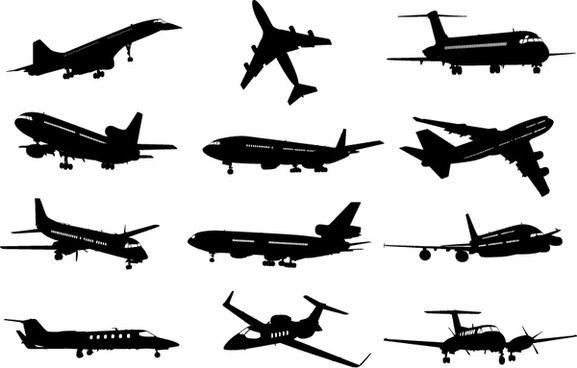
\includegraphics[width=1\textwidth]{cover}
\end{center}

\graphicspath{ {./market_trade/} }

\pagebreak

\tableofcontents

\listoffigures

\pagebreak

\section{Introduction}

This document will dive into the market analysis of the current commercial aircraft market and recommend baseline requirements (passenger count, range, and cruise speed) for an electric, fuel cell, or hybrid transport aircraft. This analysis will focus on current widebody, narrow body, regional jet, and regional turboprop aircraft. 

\section{Section 1}

Section text

\subsection{A subsection}

The figure below shows PAX vs. Range, with each marker sized by deliveries of each airplane. Note that there is a quasi-linear relationship between PAX and Range. THis relationship is described by equation \ref{eq:1}. Note that the error in slope is $\pm 5.7 [NM/PAX]$.

\begin{figure}[h]
\begin{center}
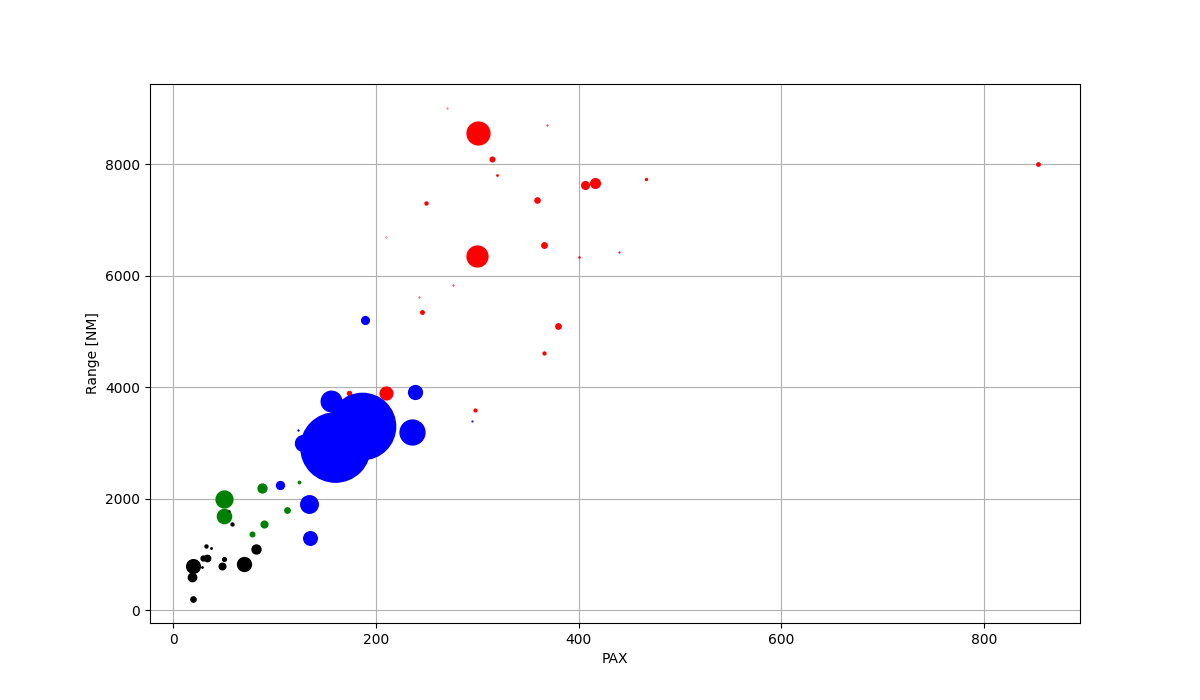
\includegraphics[width=1\textwidth]{pax_v_range}
\end{center}
\caption{PAX vs. Range}
\end{figure}

\begin{equation} \label{eq:1}
R = 18.3*PAX
\end{equation}

\begin{figure}[h]
\begin{center}
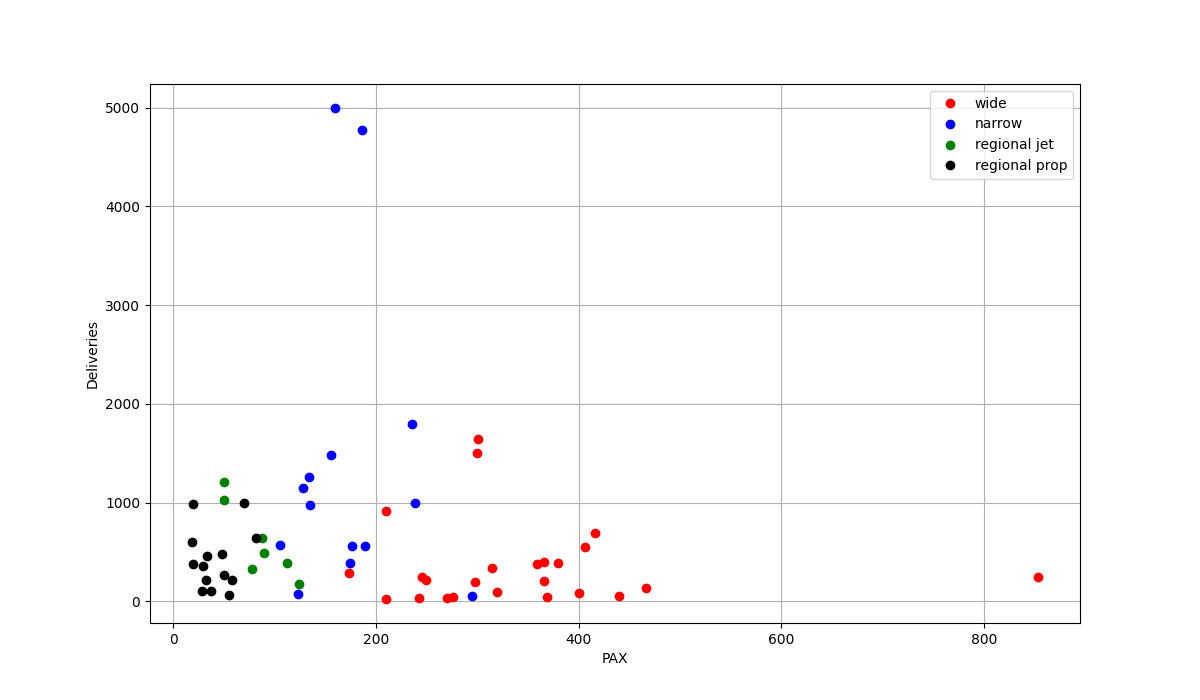
\includegraphics[width=1\textwidth]{pax_v_deliveries}
\end{center}
\caption{PAX vs. Deliveries}
\end{figure}

\subsubsection{A sub subsection}

Sub subsection text

\subsection{Conclusion}

Conclusion text

\pagebreak

\begin{thebibliography}{9}
\bibitem{latexcompanion} 
authors. 
\textit{name}. 
place, year.
\end{thebibliography}

\end{document}
